\chapter{Pendahuluan}
\label{chap:pendahuluan}

\section{Latar Belakang}
\label{sec:latar belakang}

Twitter adalah layanan jejaring sosial online yang memungkinkan pengguna memposting pesan berbasis teks hingga 140 karakter. Pengguna Twitter menyebutnya sebagai \textit{tweet}. \textit{Tweet} ini akan meneruskan pesan singkat yang ditujukan ke semua \textit{follower} suatu akun\footnote{Dusty Reagan, \textit{Twitter Application Development For Dummies}, Wiley, 2010, page 7}.\textit{Follow} adalah salah satu istilah dalam Twitter yang bertujuan untuk mengikuti aktivitas \textit{tweet} suatu akun. Sedangkan cara seseorang untuk dapat memberi rujukan kepada akun Twitter yang lainnya adalah dengan cara \textit{reply} atau lebih dikenal dengan nama \textit{mention}\footnote{Dusty Reagan, \textit{Twitter Application Development For Dummies}, Wiley, 2010, page 9}. Sebagai contoh ada akun bernama @kviniink mem-\textit{follow} @infobdg untuk mengetahui perkembangan apa saja yang tejadi di kota Bandung. Lalu akun @kviniink ingin bertanya tentang info mall yang ramai di Bandung, maka akun @kviniink membuat \textit{mention tweet} yang berisikan "@infobdg Halo saya ingin bertanya apa saja mall yang sedang ramai di Bandung yah?".

\textit{Twitter bot} adalah akun Twitter yang secara otomatis menyelesaikan suatu perintah yang diberikan. \textit{Twitter bots} memiliki fitur untuk  mengingatkan tentang suatu event melalui Twitter, seperti seseorang telah berhenti memfollow suatu akun\footnote{Dusty Reagan, \textit{Twitter Application Development For Dummies}, Wiley, 2010, page 59}. Salah satu yang menarik dari \textit{Twitter bots} ini adalah Twitter membuatnya agar didukung untuk pesan teks(\textit{text messaging}). Jadi \textit{Twitter bot} dapat memanfaatkan pesan teks untuk memungkinkan akun menyelesaikan tugas atau perintah dari ponsel mereka.

KIRI API adalah aplikasi pihak ketiga yang memungkinkan \textit{programmer} mendapatkan data tentang info jalur transportasi publik. Twitter API adalah aplikasi pihak ketiga yang memungkinkan \textit{programmer} melakukan manipulasi dan pengolahan data di Twitter. Dengan memanfaatkan KIRI API dan Twitter API penulis akan membuat program yang dapat membalas \textit{tweet} untuk mencari jalur transportasi publik. Program yang dibuat akan bersifat \textit{real time} sehingga jika seseorang melakukan mention kepada bot pencari jalur maka bot akan menangkapnya dan membalas mention tersebut berupa jalur yang harus ditempuh. Contoh dari jalannya program adalah ketika akun bernama @kviniink melakukan \textit{mention} kepada @kiriupdate untuk bertanya jalur transportasi publik "@kiriupdate #find bip to ip". Maka Twitter bot @kiriupdate akan mendengarkan mention dari akun @kviniink lalu mention tersebut akan diolah oleh server dan akan di-reply dengan tweet "@kviniink istana plaza to bandung indah plaza", "@kviniink Walk about 135 meter from your starting point to Jalan Aceh." , "@kviniink Take angkot Ciroyom - Antapani at Jalan Aceh, and alight at Jalan Pajajaran about 3.6 kilometer later.", "@kviniink Walk about 93 meter from Jalan Pajajaran to your destination.". Karena keterbatasan 140 karakter maka tweet akan dipecah sesuai dengan instruksi yang dikirimkan dari KIRI API.

\begin{figure}
	\centering
		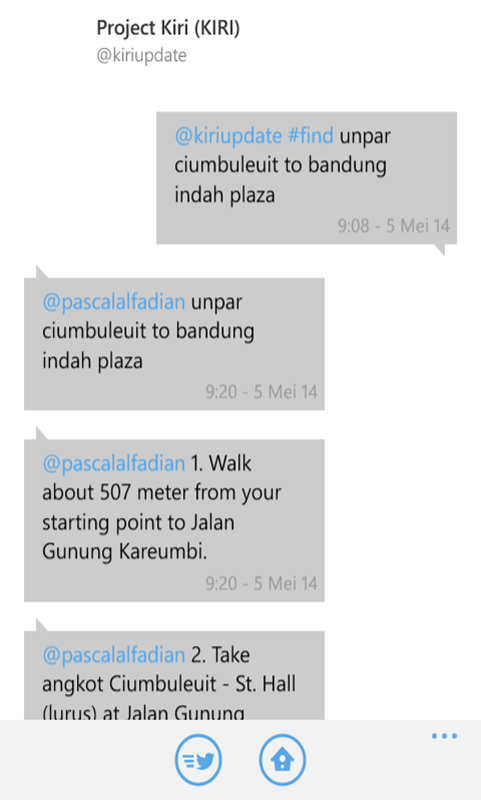
\includegraphics{C:/Users/Kvin/git/Skripsi/doc/DokumenSkripsi/Template Skripsi FTIS v7/Gambar/contoh 1.1.png}
	\caption{Gambar 1.1}
	\label{fig: Gambar 1.1}
\end{figure}


\section{Rumusan Masalah}
Mengacu kepada deskripsi yang diberikan, maka rumusan masalah pada penelitian ini adalah:
\begin{itemize}
	\item Bagaimana membuat \textit{Twitter bot} untuk mencari jalur transportasi publik?
	\item Bagaimana membuat \textit{Twitter bot} untuk dapat merespon secara real time?
	\item Bagaimana memformat petunjuk rute perjalanan dalam keterbatasan tweet 140 karakter?
\end{itemize}

\section{Tujuan}
Tujuan dari penelitian ini adalah:
\begin{itemize}
	\item Membuat aplikasi \textit{Twitter bot} untuk mencari jalur transportasi publik.
	\item Membuat aplikasi Twitter yang bekerja secara \textit{real time}.
	\item Membuat algoritma untuk memecah instruksi dari KIRI API dan mengubahnya ke dalam bentuk tweet.
\end{itemize}

\section{Deskripsi Perangkat Lunak}
Perangkat lunak akhir yang akan dibuat memiliki fitur setidaknya sebagai berikut:
\begin{itemize}
	\item Mendengarkan mention dari akun Twitter.
	\item Perangkat lunak dapat membaca \textit{input} yang diberikan oleh user melalui \textit{tweet}.
	\item Perangkat lunak dapat mencari jalur yang diberikan dengan memanfaatkan KIRI API.
	\item Perangkat lunak dapat memberikan hasil/\textit{output} berupa \textit{tweet} yang dikirimkan kepada user.
	\item Perangkat lunak dapat berjalan sebagai server yang berjalan terus menerus hingga program dihentikan.
\end{itemize}

\section{Rencana Kerja}
Rencana kerja untuk menyelesaikan skripsi ini:
\begin{itemize}
	\item Pada saat mengambil kuliah AIF401 Skripsi 1
	\begin{enumerate}
		\item Melakukan studi literatur, antara lain:
		\begin{itemize}
			\item KIRI API,
			\item REST API Twitter (https://dev.twitter.com/docs/api/1.1),
			\item Streaming API Twitter (https://dev.twitter.com/docs/api/streaming).
		\end{itemize}
		\item Mempelajari pembuatan server dalam bahasa Java.
		\item Mempelajari bahasa Java dalam membuat sebuah server.
		\item Mencoba membuat \textit{Twitter Bots} sederhana.
		\item Membuat laporan dalam bentuk skripsi.
		\item Melakukan analisis terhadap teori-teori yang sudah dipelajari, guna membangun perangkat lunak yang dimaksud.
	\end{enumerate}
	\item Pada saat mengambil kuliah AIF401 Skripsi 2
	\begin{enumerate}
		\item Merancang perangkat lunak \textit{Twitter bots}.
		\item Mengimplementasi perangkat lunak \textit{Twitter bots}.
		\item Mengimplementasikan pembangkit \textit{Twitter bots}. 
		\item Melakukan pengujian dan eksperimen.
		\item Membuat dokumentasi skripsi.
	\end{enumerate}
\end{itemize}